\chapter{Wybrane zagadnienia rzeczywistości rozszerzonej}
\label{ch:zagadnienia}
Aby zagłębić się w temat rozszerzonej rzeczywistości trzeba przede wszystkim zrozumieć czym jest rzeczywistość oraz zdefiniować pojęcia które są używane z tym zagadnieniem. Oprócz tego zostanie opisana historia powstania wirtualnych światów, dotycząca zarówno pierwszych urządzeń jak i wyobrażenia wirtualnego świata przez twórców filmów, a także zostanie opisany świat wirtualny z którego każdy może skorzystać i to już od wielu lat. W tym rozdziale opisano szczegółowo rozdzielenie różnych rodzajów rzeczywistości oraz na podstawie zebranych danych zostały wysunięte wnioski dotyczące potencjału technologii.

\section{Historia kreowania rzeczywistości}
\label{sec:historia}
Rzeczywistość według słownika jest to coś co istnieje naprawdę, bądź sytuacja lub warunki, w których ktoś żyje, coś się odbywa~\cite{sjp1}. Rozróżnienie tych dwóch definicji jest kluczowe ze względu rozszerzonej rzeczywistości. Rozszerzona rzeczywistość jest to tworzenie nowej formy rzeczywistości poprzez krzyżowanie obiektów rzeczywistych i cyfrowych. Z tego punktu widzenia można zauważyć że według drugiej definicji, rozszerzona rzeczywistość jest częścią rzeczywistości, w szczególności jeśli interakcja pomiędzy światami jest częścią czyjegoś codziennego życia. W przypadku pierwszej definicji, rozróżnienie jest bardziej wyraźne - to o czym mowa musi być prawdziwe, istnieć naprawdę. Z racji tego że na moment pisania tej pracy, integracja pomiędzy światami wirtualnymi oraz rzeczywistymi nie jest wystarczająco komfortowa aby mówić o użytkowaniu jej na równi z światem rzeczywistym, w dalszej części pracy jako rzeczywistość, przyjmuje się pierwszą definicje~\cite{XR}. Typy rozszerzonej rzeczywistości wraz z ich definicjami są przedstawione w sekcji~\ref{sec:rodzaje}, jednak z perspektywy historii, wszystko zaczęło się od jednego typu nazywanego wirtualną rzeczywistością - w skrócie VR (z ang. Virtual Reality). Pierwszym urządzeniem pozwalającym użytkownikowi na zajrzenie do wirtualnego świata, a konkretnie tworzenie złudzenia przebywania w innym miejscy jest Sensorama. Produkt ten został stworzony w 1962 roku przez Mortona Heiliga. Projekt ten powstał przed grafiką komputerową w związku z czym bazował na wyświetlaniu filmów jako obrazu. Zaledwie trzy lata później Ivan Sutheraland nazywany również ojcem grafiki komputerowej, pokazał maszynę do generowania wirtualnej rzeczywistości o nazwie Ultimate Display. Niestety była ona dużych rozmiarów jak i wagi, w związku z czym musiała być przymocowana do sufitu. W 1977 roku postęp technologiczny trwa, rozwijając nie tylko komputery ale także technologię VR - Dan Sandin stworzył pierwszy kontroler pozwalający użytkownikowi na interakcje ze światem wirtualnym w postaci rękawicy. Jest to początek dla projektów prezentowanych w dalszej części tej pracy. Wraz z latami osiemdziesiątymi powstały pierwsze urządzenia typu kinect, czyli pozwalające na kontrolowanie oraz interakcję ze światem przy pomocy kamery śledzącej nasze ciało. Jednak dopiero lata dziewięćdziesiąte pozwoliły na użytek technologii w stopniu wystarczającym aby nadawał się on do użytku w branży rozrywkowej. Wirtualna rzeczywistość przeżywa swój prawdziwy rozkwit po raz pierwszy, a to za sprawą powstania firm produkujących pierwsze gogle i rękawice do  wykorzystania w VR, zaprezentowaniu pierwszego urządzenia dla konsumentów którzy mogli korzystać ze swojego ciała w świecie wirtualnym przy użyciu wielu czujników oraz zakupie limitowanych zestawów, a także odkrycie potencjału przez branże rozrywkową, próbującą wprowadzić na rynek liczne produkty. Wzmożone zainteresowanie przyczyniło się również do powstania wielu filmów związanych z tym tematem co jeszcze bardziej pogłębiło zainteresowanie wśród ludzi. Wyobrażenia z filmów jednak odstają znacząco od możliwości technologicznych, a sam rozwój technologii nie jest tak szybki. Z tego oraz wielu innych powodów zainteresowanie normuje się aż do czasu pojawienia się na rynku Oculus Rift  w 2011 roku, który na nowo intryguje ludzi oraz pogłębia ogólne zainteresowanie technologią VR. Więcej na temat googli Oculus oraz innych urządzeń aktualnie znajdujących się na rynku jest powiedziane w sekcji~\ref{sec:okulary}~\cite{historia}.
  
\section{Wpływ kultury na rozwój technologii}
\label{sec:wplyw}
Od dawna wiadomo że rozwój technologii oraz kultura idą ze sobą w parze. Technologia ma wpływ na twórców oraz artystów, pozwalając im tworzyć nowe, bardziej kreatywne wizje przyszłości, jednocześnie dostarczając lepszych do tego środków, a na podstawie tej twórczości wielu naukowców bazowało się tworząc przełomowe wynalazki, takie jak samo prowadzące się samochody czy telekomunikację cyfrową. Również z technologią VR nie było inaczej. W poniższej sekcji zostanie przedstawione jak twórcy kinematografii prezentowali świat wirtualny, jakie to ma skutki na technologię z której teraz korzystają ludzie a także zostanie pokazany świat wirtualny który był dostępny zanim ludzkość odkryła elektryczność~\cite{wynalazki}.

	\subsection{Kinematografia}
	\label{subsec:kino}
	Wśród pozycji filmowych które zdecydowanie miały wpływ na postrzeganie wirtualnej rzeczywistości znajduję się kilka klasyków. Przede wszystkim warto wspomnieć o filmie \textit{Tron}, który zadebiutował w 1982 roku. Film ten pomimo fabuły ściśle powiązanej z technologią, pokazujący losy programisty przeniesionego do pamięci komputera. Kolejną ważną rolą tego filmu było szerokie zastosowanie grafiki komputerowej. W latach dziewięćdziesiątych wraz z rozpowszechnieniem się technologii, temat VR stał się dużo bardziej popularny co również można zaobserwować na podstawie tworzonych filmów. To właśnie w tym okresie powstały produkcje takie jak \textit{Johnny Mnemonic}, pokazujący możliwość przenoszenia danych przy pomocy umysłu, \textit{Kosiarz umysłów} - czyli ekranizacja powieści Stephena Kinga, w której wygenerowano komputerowo cyberprzestrzeń, pobudzając wyobrażenie zastosowania tej technologii w rzeczywistości i przede wszystkim \textit{Matrix}. Kultowa pozycja pokazująca ludzi zamkniętej w wirtualnej rzeczywistości którzy sami nie są tego świadomi z powodu realizmu który jest prezentowany - czyli dokładnie to co jest założeniem wirtualnej rzeczywistości. W filmach tych prezentuje się wiele metod łączenia umysłów wraz z technologią co nie wątpliwie było inspiracją dla wielu osób~\cite{filmy}. Z nowszych pozycji niewątpliwie należy wspomnieć o filmie \textit{Ready Player One}, który pokazuję wizję wirtualnego świata, realnego lecz jednocześnie z elementami dostępnymi tylko w środowisku wirtualnym. Film ten bazuje na wielu elementach technologicznych  dostępnych w chwili obecnej na rynku, jednak nie zintegrowanych ze sobą a przede wszystkim bez powszechnego dostępu co mogłoby pozwolić na zintegrowanie użytkowników ze światem wirtualnym. Jest on dla wielu wizją tego w jakim kierunku zmierza technologia oraz integracja wielu urządzeń takich jak bieżnie pozwalające na przemieszczanie się w każdym kierunku, realna odczucia całego ciała przy wykorzystaniu odpowiednich kombinezonów no i oczywiście kontrola oraz interakcja przy wykorzystaniu rękawic oraz ciała użytkownika~\cite{p1}. Wszystkie te wizje sprawiają że użytkownicy pragną coraz bardziej realnych doznań oraz interakcji, a także możliwości osiągnięcia wykonania zadania bez konieczności wychodzenia z domu. Oczywiście realizując to, każdy wie że znajduje się w świecie wirtualnym z powodu świadomego przejścia. Gdyby jednak nawet ktoś się obudził w takiej przestrzeni nieświadomy tranzycji pomiędzy rzeczywistościami, łatwo można to określić na podstawie zamontowanych kontrolerów, kombinezonów czy okularów które wyczuwa się na ciele, a także wad elementów graficznych którym wciąż brakuje wystarczającego realizmu. Istnieje jednak metoda która pozwala temu zapobiec, która może posłużyć jako przykład wirtualnego świata w trybie pojedynczego gracza.
	
	\subsection{Marzenia senne}
	\label{subsec:sny}
	Podczas analizy sztucznej rzeczywistości ważnym punktem jest sen, a konkretnie marzenia senne. Przeciętnie człowiek potrzebuje od siedmiu do dziewięciu godzin snu dziennie w cyklu monofazowym, czyli gdy zasypia się i budzi tylko raz dziennie. W tym czasie występują marzenia senna, potocznie nazywane snami. W zależności od osoby swoje sny można pamiętać bądź nie, jednak warto podkreślić że każda osoba ma sny - zapamiętywanie marzeń sennych, tak jak z każdą inną umiejętność można wytrenować, aby pamiętać więcej szczegółów, miejsc oraz wydarzeń. Mając to na uwadze należy sprecyzować czym one właściwie są. Marzenia senne są serią myśli, obrazów oraz odczuć które dana osoba przeżywa w swoim umyśle w trakcie snu. Nie jest to też dowolny moment w trakcie spania. Sen odbywa się w cyklach, które średnio trwają dziewięćdziesiąt minut i składają się z kilku faz takich jak sen przejściowy, głęboki sen czy faza ruchu gałek ocznych - w każdej fazie można śnić jednak to w tej ostatniej najczęściej występują marzenia senne które są rzeczywiste i realistyczne - w wielu przypadkach nie sposób ich odróżnić od rzeczywistości. Faza ta nazywana fazą REM ( z ang. Rapid Eye Movement) jest etapem snu w którym nasz umysł wprowadzany jest w specjalny stan aby móc osiągnąć ten efekt. Przede wszystkim warto zauważyć że etap ten charakteryzuje się wysoką aktywnością mózgu, porównywalną z tą gdy osoba jest przytomna, sprawia to że bardzo łatwo przerwać ten etap i wybudzić się w trakcie snu. Oprócz tego w naszym mózgu przepływa wiele impulsów przez różne jego obszary, niejako testując połączenia, co jest podejrzewane jako przyczynę tworzenia się w naszym umyśle obrazów, doznań dźwiękowych oraz ruchowych. Aby jednak impulsy nie zostały wysłane do mięśni w ciele, w trakcie snu występują ich atonia, czyli zniesienia napięcia mięśniowego. W ten sposób w trakcie gdy ciało leży nieruchomo, w odpowiednim momencie snu dochodzi do symulacji świata w umyśle, w trakcie której osoba może przeżywać wydarzenia które mogą być nawet nie możliwe do zrealizowania w świecie rzeczywistym. Interesującym jest więc fakt, że większość osób zdaje sobie sprawę tuż po przebudzeniu, że wydarzenia które przed chwilą miały miejsce były jedynie marzeniami sennymi - nie były one rzeczywistością. Dzieje się tak za sprawą kory przedczołowej - części mózgu która jest odpowiedzialna za myślenie logiczne, planowanie ruchów i działań, oraz pełni funkcje w działaniu pamięci roboczej. Kora przedczołowa jest jednym z obszarów mózgu który w trakcie snu wytwarza jedynie minimalną aktywność co sprawia że gdy marzenia senne zaczynają się w zupełnie innym miejscu od lokalizacji danej osoby, z ludźmi których dana osoba nie zna, bądź wręcz nie powinno ich tam być, jak na przykład osoby zmarłe bądź znajdujące się w innym miejscu na ziemi, mózg tego nie kwestionuje - przyjmuje że to co się dzieje jest zupełnie normalne. Za sprawą tych mechanizmów, niejako każda osoba codziennie ma dostęp to sztucznej rzeczywistości w której może znaleźć się w dowolnym miejscu, z dowolnymi osobami, przeżywając zdarzenia które mogą być nawet sprzeczne z prawami fizyki. 
	
W obecnych czasach jeżeli mówimy o wirtualnej rzeczywistości, nie myślimy o maszynie takiej jak Sensorama, która jedynie wyświetlała filmy. Poruszając ten temat myślimy o kontrolowanym środowisku w którym użytkownik ma możliwość interakcji z otoczeniem a nawet jego kontrole. W rozumieniu marzeń sennych, zwykłe sny są tym czym Sensoroma jest dla współczesnej technologii VR. Świadome śnienie natomiast odkrywa pełną moc możliwości która kryje się w tym naturalnym ludzkim procesie. Aby podjąć próbę świadomego snu należy oczywiście najpierw być w stanie pamiętać swoje zwyczajne marzenia senne. Świadomy sen jest to rodzaj snu w którym osoba śniąca zdaje sobie sprawę z tego że znajduje się w świecie marzenia sennego. Istnieje wiele metod które pozwalają osiągnąć ten stan, jednak ogólnie mówiąc sprowadzają się one do kwestionowania rzeczywistości, dzięki czemu możemy niejako zakodować ten proces w podświadomości. Tak jak wspomniano kora przedczołowa odpowiadająca za logiczne myślenie nie wykazuje dużej aktywności w trakcie snu, jednak nie jest ona całkowicie nieaktywna, dzięki czemu nadal można ją wykorzystać nawet podczas snu. Jeżeli osoba zakwestionuje rzeczywistość w trakcie marzenia sennego, na przykład poprzez złamanie praw fizyki, i rezultat takiego testu pokaże niemożliwe rezultaty w świecie rzeczywistym, osoba taka odzyskuje świadomość. Często w początkowych próbach dochodzi w tym momencie do wybudzenia, ponieważ jest to niejako przełamanie naturalnego mechanizmu organizmu. Z praktyką jednak dochodzi do stabilizacji świata a dzięki uzyskaniu świadomości, dochodzi do uzyskania kontroli nad naszym umysłem, czyli marzeniem sennym. W ten oto sposób mózg od wewnątrz, bez dodatkowych urządzeń i kontrolerów, generuje własny świat ''wirtualny``, odtwarzając bodźce wzrokowe, słuchowe, dotyku oraz wszystkie inne zmysły. Osoba kontrolująca ma pełną kontrole nad własnym ciałem i z jej perspektywy świat w którym się znajduje dostarcza tych samych bodźców co świat rzeczywisty, a dla osób które potrafią kontrolować otoczenie, bodźców możliwych do doświadczenia jedynie poza światem rzeczywistym takich jak np. latanie czy teleportacja~\cite{sen2}~\cite{sen1}. 		
	
\section{Rodzaje rzeczywistości}
\label{sec:rodzaje}
Umiejętność świadomego snu jest treningiem przejęcia kontroli nad naturalnym procesem śnienia występującym u każdej osoby, pozwalając niejako doświadczyć tego dokąd technologia wirtualnej rzeczywistości zmierza - bezbłędnego odwzorowania świata rzeczywistego, przy dostarczeniu do mózgu wszystkich bodźców w taki sposób aby osoba użytkująca odniosła pełne wrażenie realizmu otoczenia. Mając to na uwadze, w tej sekcji zostanie zdefiniowane czym jest rozszerzona rzeczywistość, jakie rodzaje rzeczywistości obejmuje ten termin oraz wyjaśnić dokładnie pojęcie wirtualnej rzeczywistości które było używane w tym rozdziale. 
	%\subsection{XR}
%	\label{subsec:xr}

	Akronim XR (z ang. Extended Reality) jest tłumaczony na język polski na wiele sposobów takich jak rzeczywistość rozszerzona ( w odróżnieniu od rozszerzonej rzeczywistości) czy rzeczywistość skrzyżowana. W praktyce jednak najczęściej używa się skrótów angielskich które pozwalają jednoznacznie określić zagadnienie. Termin XR jest używany jako ogólne wyrażenie wszystkich technologii wpływających na zmianę rzeczywistości, które mogą zostać użyte razem bądź pojedynczo. W związku z tym aplikacje mieszające obiekty wirtualne z rzeczywistymi które mogą dowolnie przełączać się pomiędzy tym światem a światem czysto wirtualnym są określane tym terminem, jak i każdy z projektów wykorzystujących tylko jeden typ technologii zmiany rzeczywistości. W chwili pisania tej pracy terminem XR określa się zbiór technologi wirtualnej rzeczywistości, rozszerzonej rzeczywistości a także mieszanej rzeczywistości, jednak określenie to powstało w celu włączenia do jednego określenia również wszystkich terminów które mogą zostać stworzone w przyszłości~\cite{terms}.
	%\subsection{VR}
	%\label{subsec:vr}
	
	Pojęcie wirtualnej rzeczywistości określa się skrótem VR ( z ang. Virtual Reality) i definiuje ono część technologii kreowania rzeczywistości w pełni wirtualnej - oznacza to że nie znajdują się w niej żadne elementy świata rzeczywistego. Jeżeli elementy te miały by być prezentowane w takim środowisku muszą one zostać wygenerowane komputerowo. Celem VR jest stworzenie jak najbardziej realistycznych i rzeczywistych odczuć dla użytkownika niezależnie od środowiska w jakim się znajduje. Aby to osiągnąć niezbędna jest symulacja która wpływa na wszystkie zmysły użytkownika. Dlatego też firmy pracują nad coraz bardziej realistycznymi i dokładnymi rozwiązaniami które pozwalają na głębszą imersję w świat wirtualny. Jest to również jednym z głównych powodów dla których zostały stworzone rękawice-kontrolery. Pozwalają one na większą swobodę oraz bardziej naturalny ruch w  wygenerowanej przestrzeni, zapewniając lepsze odczucia oraz komfort podczas przebywania w świecie wirtualnym. Nad zapewnieniem realizmu, oprócz metody kontroli środowiska, składa się wiele innych czynników. W tym celu powstają specjalne kombinezony które odwzorowują ruch całego ciała, bieżnie które pozwalają się poruszać w VR, dzięki naturalnemu przemieszczeniu się, które za sprawą bieżni odbywa się w miejscu w świecie rzeczywistym, okularów które pozwalają wyświetlać przed oczami środowisko wirtualne, starając się odwzorować głębię oraz wiele innych urządzeń. Ilość urządzeń oraz metod imitacji pokazuje jak skomplikowanym problemem jest odwzorowanie rzeczywistości, a wszystko to musi odbywać się niezwykle płynnie ponieważ mózg człowieka nie rozróżnia rzeczywistości od świata wirtualnego. Oznacza to że jeżeli bodźce wzrokowe nie pokrywają się z bodźcami słuchowymi dochodzi do tak zwanego zjawiska choroby lokomocyjnej. Sprawia to że przebywania w wirtualnym świecie przez długi okres czasu może doprowadzić do dyskomfortu dla użytkownika. Aby zapobiec tego rodzaju problemom równie ważnym jest dokładna znajomość fizjologii człowieka, co prowadzi do współpracy wielu działów nauki w celu stworzenia prawdziwie realistycznych produktów. Pomimo wielu przeszkód jak przedstawiono w sekcji~\ref{sec:historia}, wirtualna rzeczywistość była pierwszą wizją naukowców którą starano się zrealizować - pomimo dużych nakładów pracy w celu zapewnienia realistyczności, niesie ona za sobą wiele możliwości zarówno w biznesie jak i życiu codziennym, co sprawia że dla wielu firm jest to możliwość realizowania własnej wizji wirtualnej przyszłości~\cite{terms}~\cite{chorobaVR}.
	%\subsection{AR}
	%\label{subsec:ar}
	
	Kolejnym terminem wchodzącym w skład XR jest rozszerzona rzeczywistość, bądź też nazywana rzeczywistością poszerzoną. Skrótowo zapisuje się ją jako AR (z ang. Augmented Reality). Podobnie brzmiąca do XR w szczególności w języku polskim jest częstym powodem dla którego powszechnie używa się skrótów angielskich mówiąc o tym obszarze technologii. AR jak nazwa wskazuje poszerza rzeczywistość zamiast ją zastępować tak jak to miało w przypadku VR. Oznacza to że do elementów świata rzeczywistego zazwyczaj pozyskanych przy pomocy obrazu z kamery, wyświetlanych poprzez wybrane źródło obrazu o których mowa w rozdziale~\ref{ch:prezentacja}, są dodawane elementy stworzone przy pomocy grafiki komputerowej, zazwyczaj trójwymiarowe. Technologia ta dzięki wykorzystaniu w dużej mierze świata rzeczywistego jest łatwiejsza w użytkowaniu a jej zastosowanie jest powszechnie stosowane w wielu branżach. W szczególności duży sukces technologia ta odniosła gdy wykorzystano ją do stworzenia popularnej gry na smart-fony \textit{Pokemon Go}, która przy wykorzystaniu geolokalizacji oraz AR zapewniała realistyczne doświadczenia łapania stworzonych trójwymiarowych postaci w świecie rzeczywistym~\cite{terms}. Podgląd interfejsu aplikacji obrazujący wykorzystanie technologii AR  w \textit{Pokemon Go} pokazuje rysunek~\ref{fig:pokemon}.
	
\begin{figure}[h]
\centering
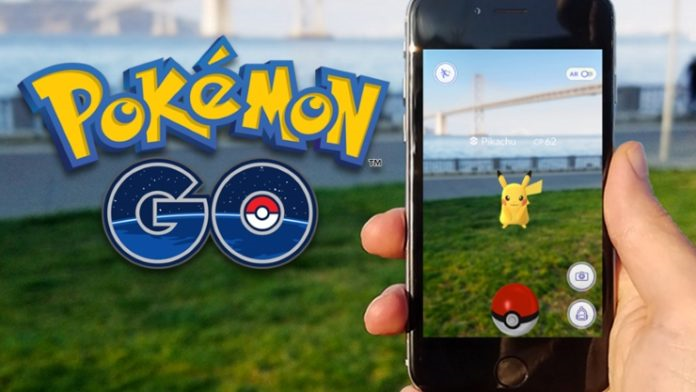
\includegraphics[scale=0.6]{pokemon}
\captionsource{Interfejs aplikacji \textit{Pokemon Go} wykorzystujący AR.}{\url{https://gameradar.pl/aktualizacja-pokemon-go-utrudnia-lapanie-pokemonow/}}
\label{fig:pokemon}
\end{figure}

	%\subsection{MR}
	%\label{subsec:mr}	
	
	Mieszana rzeczywistość, czyli MR (z ang. Mixed Reality) jest terminem który prawdopodobnie jest najczęściej błędnie używanym wśród zagadnień związanych z XR. Mieszana rzeczywistość podobnie jak AR wykorzystuje do działania zarówno świat rzeczywisty jak i stworzony komputerowo, jednak w odróżnieniu od AR nastawiony jest głównie na interakcję pomiędzy tymi światami. Obiekty tworzone cyfrowo wyświetlane w świecie rzeczywistym mogą być modyfikowane i wpływać na środowisko rzeczywiste które jest wyświetlane jak i obiekty rzeczywiste mogą zostać przeniesione do świata wirtualnego. Interakcja ta i zastosowanie jest niejako technologią przyszłości, wizją producentów, ponieważ do tej pory nie ma łatwo dostępnych produktów które by wykorzystywało ten rodzaj XR, natomiast istnieją takie rozwiązania dla biznesu oraz w ośrodkach badawczych, które prawdopodobnie staną sie bardziej dostępne wraz z rozwojem tej technologii oraz ulepszonych rozwiązań w innych dziedzinach technologicznych takich jak grafika komputerowa, prędkość przesyłania czy przetwarzania danych~\cite{terms}.
%\section{Potencjał technologii}
%\label{sec:potencjal}

Rozwiązania XR przebyły długą drogę od czasu powstania pierwszej wizji tego typu rozwiązania. Obecnie istnieje wiele urządzeń które powszechnie korzystają z XR zarówno na użytek prywatny, branży rozrywkowej oraz w celu usprawnienia procesów biznesowych. Niemniej jednak dopiero są opracowywane rozwiązania które mogłyby zapewnić większą przenośność tego typu urządzeń, sprawniejsze połączenie i przede wszystkim realizm. Wykorzystanie w życiu codziennym staje się coraz bardziej powszechne, w związku z tym można też się  spodziewać ulepszeń produktów zarówno pod względem sprzętu jak i oprogramowania a także dostępności tych produktów przy mniejszym koszcie. Można być pewnym że technologia ta nie przestanie się rozwijać, znajdując coraz to nowe zastosowania, inwestorów a także twórców którzy wprowadzając większą liczbę produktów na rynek, tworzą większe zainteresowanie wśród społeczności. Pytanie stawiane przez technologię XR to nie czy ta technologia ma przyszłość, a kiedy stanie się ona powszechnie stosowana. W dalszych częściach tej pracy zostaną pokazane sposoby w jakich obecnie przedstawiane i wykorzystywane są opisywana do tej pory technologie, a także zostanie szczegółowo opisany temat rękawic-kontrolerów, urządzenia które nie jest standardem wśród kontrolerów na rynku dla pojedynczych konsumentów VR, jednak już jest wykorzystywany w biznesie a także przewidywany jest jako kontroler przyszłości~\cite{terms}.

